\documentclass[10pt]{beamer}

\usetheme[progressbar=foot]{metropolis}
% font options
\usefonttheme{professionalfonts}
\usepackage{appendixnumberbeamer}

\usepackage{booktabs}
\usepackage[scale=2]{ccicons}

\usepackage{pgfplots}
\usepgfplotslibrary{dateplot}

\usepackage{lmodern}

\usepackage{cancel}

\usepackage{color}

\usepackage{subcaption}

\usepackage{xstring}

\usepackage{xspace}
\usepackage{siunitx}
\sisetup{per-mode=fraction, inter-unit-product={}\cdot{}}
\DeclareSIUnit\particles{particles}

\newcommand{\themename}{\textbf{\textsc{metropolis}}\xspace}

\usepackage[usestackEOL]{stackengine}

\title{\color{berkeleyblue} Variable Eddington Factor Method with Hybrid Spatial Discretization}
\subtitle{\normalsize International Conference on Transport Theory \\ Novel Numerical Methods}
% \date{\today}
\date{October 19, 2017}
\author{Samuel S. Olivier$^1$, Jim E. Morel$^2$}
\institute{$^1$Department of Nuclear Engineering, University of California, Berkeley \\$^2$Department of Nuclear Engineering, Texas A\&M University \\ \\ 
\scriptsize
% \url{https://github.com/smsolivier/EddingtonAcceleration.git} \\ 
\vfill

\includegraphics[height=1cm]{berkeley.eps}
% \titlegraphic{\hfill
\includegraphics[height=1.5cm]{nuen-logo.png}}
}

\newcommand{\SN}{S$_N$\xspace}
\renewcommand{\vec}[1]{\bm{#1}} %vector is bold italic
\newcommand{\vd}{\bm{\cdot}} % slightly bold vector dot
\newcommand{\ud}{\mathop{}\!\mathrm{d}} % upright derivative symbol
\newcommand{\pderiv}[2]{\frac{\partial #1}{\partial #2}}
\newcommand{\dderiv}[2]{\frac{\ud #1}{\ud #2}}
\newcommand{\edd}{\langle \mu^2 \rangle} 
\newcommand{\rell}{^\ell} % raise to ellth power 
\newcommand{\relll}{^{\ell+1}} % raise to ell + 1 th power 
\newcommand{\rellh}{^{\ell+1/2}} % raise to ell + 1/2 power
\newcommand{\bracket}[1]{\left[ #1 \right]}

\newcommand{\paren}[1]{\left(#1\right)} 
\newcommand{\br}[1]{\left[#1\right]}
\newcommand{\curl}[1]{\left\{#1\right\}}

\newcommand{\eddphi}[1]{\edd_{#1}\phi_{#1}}
\newcommand{\ALPHA}[2]{\frac{#1}{\sigma_{t,#2} h_{#2}}}

% make blocks fill 
\metroset{block=fill}

% dark background 
% \metroset{background=dark}

% color options
\definecolor{maroon}{RGB}{80,0,0}
\definecolor{berkeleyblue}{HTML}{003262}
\definecolor{calgold}{HTML}{FDB515}
\definecolor{founder}{HTML}{3B7EA1}
\definecolor{medalist}{HTML}{C4820E}
\definecolor{goldengate}{HTML}{ED4E33}
\setbeamercolor{progress bar}{fg=founder, bg=berkeleyblue!30}
\setbeamercolor{progress bar in head/foot}{fg=founder, bg=berkeleyblue!30}
\setbeamercolor{progress bar in section page}{fg=founder, bg=berkeleyblue!30}
\setbeamercolor{palette primary}{bg=berkeleyblue}

\setbeamercolor{alerted text}{fg=founder}

\setbeamertemplate{frametitle continuation}{}

\setbeamertemplate{frame numbering}[fraction]

\makeatletter
% \setlength{\metropolis@titleseparator@linewidth}{2pt}
\setlength{\metropolis@progressonsectionpage@linewidth}{1.5pt}
\setlength{\metropolis@progressinheadfoot@linewidth}{1.5pt}
\makeatother

\setbeamertemplate{block begin}
{
  \par\vskip\medskipamount%
  \IfStrEq{\insertblocktitle}{}{}{
      \begin{beamercolorbox}[colsep*=.75ex]{block title}
        \usebeamerfont*{block title}\insertblocktitle%
      \end{beamercolorbox}%
  }
  {\parskip0pt\par}%
  \ifbeamercolorempty[bg]{block title}
  {}
  {\ifbeamercolorempty[bg]{block body}{}{\nointerlineskip\vskip-0.5pt}}%
  \usebeamerfont{block body}%
  \begin{beamercolorbox}[colsep*=.75ex,vmode]{block body}%
    \ifbeamercolorempty[bg]{block body}{\vskip-.25ex}{\vskip-.75ex}\vbox{}%
}


% ---------------------------------------
\begin{document}

\maketitle

\begin{frame}[plain,noframenumbering]{Overview}
  \setbeamertemplate{section in toc}[sections numbered]
  \tableofcontents[hideallsubsections]
\end{frame}

\section{Background}

\begin{frame}{Variable Eddington Factor Method}

	% \begin{itemize}
	
		% \item 
		One of the first nonlinear methods for accelerating source iterations

		% \item 
		Use \SN to iteratively create a transport-informed drift diffusion solution  

		% \item 
		Produces 2 solutions: one from \SN and one from drift diffusion 
		\begin{itemize}
			\item Do not necessarily become identical when the iterative process converges if not consistently differenced 

			\item Solutions do converge as the mesh is refined $\Rightarrow$ built in truncation estimator 
		\end{itemize}

		Will show that the benefits outweigh producing 2 separate solutions 


	% \end{itemize}

\end{frame}

\begin{frame}{Why Nonlinear Acceleration?}

	% \begin{itemize}

		% \item 
		Classic discretizations (step, diamond) are not suitable for radiative transfer in High Energy Density Physics regime $\Rightarrow$ Discontinuous Galerkin (DG) \SN

		% \item 
		Linear acceleration of Discontinuous Finite Element \SN is somewhat problematic 
		\begin{itemize}
			\item Consistent differencing required (Adams and Martin NSE 1992)

			\item Requires the diffusion equation to be expressed in $P_1$ form which is more difficult to solve (Warsa, Wareing, Morel NSE 2002) 

			\item Partially consistent linear acceleration methods are generally difficult to develop (Wang and Ragusa NSE 2010)

		\end{itemize}

	% \end{itemize}

\end{frame}

\begin{frame}{Why Nonlinear Acceleration? (cont.)}

	% \begin{itemize}

		% \item 
		Nonlinear acceleration has relaxed consistency requirements 
		\begin{itemize}
			\item Drift diffusion acceleration equation can be discretized in any valid manner without regard for consistency with \SN  

			\item Preserves the thick diffusion limit regardless of discretization consistency as long as \SN solution becomes isotropic 
		\end{itemize}

		% \item 
		Can use VEF drift diffusion in multiphysics calculations  
		\begin{itemize}

			\item VEF drift diffusion is conservative and inexpensive (compared to an \SN sweep) 

			\item Couple drift diffusion to other physics components 

			\item Can use discretization compatible with other physics while still retaining benefits of DG \SN 

		\end{itemize}

	% \end{itemize}

\end{frame}

\begin{frame}{Motivation}

	% \begin{itemize}

		% \item 
		Mixed Finite Element Method (MFEM) is being used for high order hydrodynamics calculations (Dobrev, Kolev, Rieben SIAM 2012)

		% \item 
		MFEM is not appropriate for standard, first-order form of transport equation 

		% \item 
		$\Rightarrow$ VEF method with DG \SN discretization + MFEM drift diffusion discretization 

	% \end{itemize}

	\vfill
	\begin{alertblock}{Goals}
		
		Show Lumped Linear Discontinuous Galerkin (LLDG) \SN can be efficiently and accurately paired with MFEM drift diffusion for one group, 1D neutron transport 

	\end{alertblock}

\end{frame}

\section{Description of VEF Method}

\begin{frame}{\SN Equations}

	Planar geometry, fixed-source, 1-D, one group, neutron transport equation 
	\begin{equation*} 
		\mu \pderiv{\psi}{x} \paren{x, \mu} + \sigma_t(x) \psi(x,\mu) = 
			\frac{\sigma_s(x)}{2} \int_{-1}^1 \psi(x,\mu') \ud \mu' + \frac{Q(x)}{2}
	\end{equation*}

	\pause
	\SN angular discretization 
	\begin{equation*} \label{eq:sn}
		\mu_n \dderiv{\psi_n}{x}(x) + \sigma_t(x) \psi_n(x) = 
		\frac{\sigma_s(x)}{2} \phi(x) + \frac{Q(x)}{2} \,, \quad 1 \leq n \leq N
	\end{equation*}

	where 
	\begin{equation*}
		\phi(x) = \sum_{n=1}^N w_n \psi_n(x) \,, \quad \psi_n(x) = \psi(x, \mu_n)
	\end{equation*}

\end{frame}

\begin{frame}{Source Iteration}

	Lag scattering term 
	\begin{equation*} \label{eq:si}
		\mu_n \dderiv{}{x}\psi_n\rellh(x) + \sigma_t(x) \psi_n\rellh(x) = 
		\frac{\sigma_s(x)}{2} \phi^\ell(x) + \frac{Q(x)}{2} \,, \quad 1 \leq n \leq N 
	\end{equation*}

	\pause
	Source Iteration 
	\begin{equation*}
		\phi^{\ell+1} = \phi\rellh
	\end{equation*}

	\pause
	Slow to converge in optically thick and highly scattering systems 

\end{frame}

\begin{frame}{VEF Drift Diffusion}

	Instead, solve 
	\begin{equation*} \label{eq:drift}
	-\dderiv{}{x} \frac{1}{\sigma_t(x)} \dderiv{}{x} \bracket{\edd\rellh(x)\phi\relll(x)} + \sigma_a(x) \phi\relll(x) = Q(x) \,,
	\end{equation*}
	for $\phi\relll(x)$ using transport information from iteration $\ell+1/2$

	\pause 
	Transport information passed through the \alert{Variable Eddington Factor:}
	\begin{equation*} \label{eq:eddington} 
		\edd\rellh(x) = \frac{\int_{-1}^1 \mu^2 \psi\rellh(x, \mu) \ud \mu}{\int_{-1}^1 \psi\rellh(x, \mu) \ud \mu}
	\end{equation*}

	\begin{itemize}
		\pause
		\item Angular flux weighted average of $\mu^2$ 

		\pause
		\item Depends on angular shape of the angular flux, not its magnitude 
	\end{itemize}

	\pause
	Use $\phi\relll$ to update scattering term in \SN sweep or as final solution if converged 

\end{frame}

\begin{frame}{Acceleration Properties}

	Angular shape of the angular flux, and thus the Eddington factor, converges much faster than the scalar flux 

	Drift diffusion includes scattering 

\end{frame}

\begin{frame}{VEF Algorithm}

	\begin{figure}

		\only<1>{\def\svgwidth{.8\textwidth}\input{figs/vef_flow.pdf_tex}}%
		\only<2>{\def\svgwidth{.8\textwidth}\input{figs/vef_discretized.pdf_tex}}

	\end{figure}

\end{frame}

\section{Discretizations}

\begin{frame}{Lumped Linear Discontinuous Galerkin \SN}

	\begin{columns}

		\begin{column}{.5\textwidth}
		\vspace{.1in}
		\begin{itemize}

			\item 
			2 discontinuous, linear basis functions 

			\item 
			Cell edges uniquely defined through upwinding 

			% \item Cell centers through polynomial interpolation (in linear case it is just the average of $\psi_{i,L}$ and $\psi_{i,R}$) 

		\end{itemize}
		\end{column}
		\begin{column}{.5\textwidth}

			\begin{figure}

				\def\svgwidth{\textwidth}
				\input{figs/lldg.pdf_tex}
				% \caption{Unknowns and upwinding for an LLDG cell. }
				
			\end{figure}

		\end{column}

	\end{columns} 

	\begin{columns}
	\begin{column}{1.06\textwidth}
	\begin{itemize}

		\item 
		Within the cell, $\psi$ is a linear combination of the basis functions:
		\begin{equation*}
			\psi_{n,i}(x) = \psi_{n,i,L} B_{i,L}(x) + \psi_{n,i,R} B_{i,R}(x) \,, \quad x \in (x_{i-1/2},x_{i+1/2})
		\end{equation*}
		\item 
		Cell centers through through polynomial interpolation (evaluate at $x_i$) 

		\item 
		Linear case: average of $\psi_{n,i,L}$ and $\psi_{n,i,R}$ 

		\item Sweep through local systems 

	\end{itemize}

	\end{column}
	\end{columns}

\end{frame}

% --- alternate form of LLDG slide --- 
% \begin{frame}{LLDG}

% 	2 discontinuous, linear basis functions 

% 	Cell edges uniquely defined through upwinding 

% 	Within the cell, 
% 	\begin{equation*}
% 		\psi_{n,i}(x) = \psi_{n,i,L} B_{i,L}(x) + \psi_{n,i,R} B_{i,R}(x) \,, \quad x \in (x_{i-1/2},x_{i+1/2}) \,, 
% 	\end{equation*}
% 	Cell centers through through polynomial interpolation (evaluate at $x_i$) 

% 	Linear case $\Rightarrow$ just average of $\psi_{n,i,L}$ and $\psi_{n,i,R}$ 

% 	\vfill
% 	\begin{figure}
% 		\centering
% 		\def\svgwidth{.8\textwidth}
% 		\input{figs/upwind.pdf_tex}
% 	\end{figure}

% \end{frame}

\begin{frame}{Handling Overlap in Eddington Factor}

	For integration by parts in MFEM weak form, need:
	\begin{itemize}
		\item $\edd$ on cell boundary 
		\item $\edd(x)$ on interior of cell 
	\end{itemize}

	Cell edges: use \alert{uniquely defined, upwinded} cell edge values of $\psi$ in Gauss Quadrature 
	\begin{equation*} \label{lldg:edde}
		\edd_{i\pm 1/2} = \frac{
			\sum_{n=1}^N \mu_n^2 \psi_{n,i\pm 1/2} w_n
		}{
			\sum_{n=1}^N \psi_{n,i\pm 1/2} w_n 
		} 
	\end{equation*}

	Cell centers: use polynomial interpolation function for the angular flux 
	\begin{equation*} \label{lldg:eddi}
			\edd(x) = \frac{
				\sum_{n=1}^N \mu_n^2 \psi_{n}(x) w_n
			}{
				\sum_{n=1}^N \psi_{n}(x) w_n 
			} \,, \quad x\in(x_{i-1/2},x_{i+1/2}) 
		\end{equation*}

	\begin{itemize}
		\item Rational polynomial $\Rightarrow$ can't be integrated analytically 

		\item Preserves nonlinear spatial dependence of Eddington factor in MFEM formulation 

	\end{itemize}

\end{frame}

\begin{frame}{Constant-Linear Mixed Finite Element Drift Diffusion}

	\begin{columns}
	\begin{column}{.5\textwidth}

		\begin{itemize}

			\item Different basis functions for primary and secondary variables ($\phi$, $J$)

			\item $\phi$: constant with discontinuous jumps at the edges 

			\item $J$: linear discontinuous basis functions (same as in LLDG) 

		\end{itemize}
		
	\end{column}
	\begin{column}{.5\textwidth}

		\begin{figure}

			\def\svgwidth{\textwidth}
			%!TEX root = ./jctt.tex

\subsection{Mixed Finite Element Method VEF Drift Diffusion}
\begin{figure}
	\centering
	% \def\svgwidth{\textwidth}
	\input{figs/mfemgrid.pdf_tex} 
	\caption{The distribution of unknowns in cell $i$ for MFEM. }
	\label{fig:mfem_grid}
\end{figure}
The unknowns in an MFEM cell are depicted in Fig. \ref{fig:mfem_grid}. The scalar flux is constant within the cell with discontinuous jumps at the cell edges and the current is a linear function defined by: 
	\begin{equation} \label{eq:MFEM_current}
		J_i(x) = J_{i,L} B_{i,L}(x) + J_{i,R} B_{R,i}(x) \,, 
	\end{equation} 
where $J_{i,L/R}$ are the currents at the left and right edges of the cell and 
	\begin{subequations}
		\begin{equation}
			B_{i,L}(x) = \begin{cases}
				\frac{x_{i+1/2} - x}{h_i} \,, & x \in [x_{i-1/2}, x_{i+1/2}] \\ 
				0 \,, & \text{otherwise}
			\end{cases} \,,
		\end{equation}
		\begin{equation}
			B_{i,R}(x) = \begin{cases}
				\frac{x - x_{i-1/2}}{h_i} \,, & x \in [x_{i-1/2}, x_{i+1/2}] \\ 
				0 \,, & \text{otherwise}
			\end{cases} \,,
		\end{equation}
	\end{subequations}
are the MFEM basis functions. The spatial grid used in this step is identical to the grid used in the LLDG \SN step. 

The MFEM representation yields five unknowns per cell: $\phi_{i-1/2}$, $\phi_i$, $\phi_{i+1/2}$, $J_{i,L}$, and $J_{i,R}$. An equation for $\phi_i$ is found by integrating Eq. \ref{eq:zero} over cell $i$: 
	\begin{equation} \label{mfem:balance}
		J_{i,R} - J_{i,L} + \sigma_{a,i} h_i \phi_i = Q_i h_i \,,
	\end{equation}
where $\sigma_{a,i}$ and $Q_i$ are the absorption cross section and source in cell $i$. Equations for $J_{i,L/R}$ are found by multiplying Eq. \ref{eq:first} by $B_{i,L/R}$ and integrating over cell $i$: 
	\begin{subequations}
		\begin{equation} \label{mfem:bli}
			-\edd_{i-1/2} \phi_{i-1/2} + \edd_i \phi_i + \sigma_{t,i} h_i \left(\frac{1}{3} J_{i,L} + \frac{1}{6}J_{i,R}\right) = 0 \,,
		\end{equation}
		\begin{equation} \label{mfem:bri}
			\edd_{i+1/2} \phi_{i+1/2} - \edd_i \phi_i + \sigma_{t,i} h_i \left(\frac{1}{6} J_{i,L} + \frac{1}{3} J_{i,R}\right) = 0 \,, 
		\end{equation}
	\end{subequations}
where the fixed source has been assumed to be isotropic. The Eddington factors, $\edd_{i(\pm1/2)}$, are computed using the angular fluxes from the LLDG \SN step according to: 
	\begin{equation} 
		\edd_{i(\pm1/2)} = \frac{
			\sum_{n=1}^N \mu_n^2 \psi_{n,i(\pm1/2)} w_n 
		}{
			\sum_{n=1}^N \psi_{n,i(\pm1/2)} w_n
		} \,,
	\end{equation}
where the cell edge angular fluxes are defined by Eq. \ref{eq:downwind} and \ref{eq:upwind} and the cell centered angular flux by Eq. \ref{eq:lldg_i}. 
Eliminating $J_{i,R}$ from Eq. \ref{mfem:bli} and $J_{i,L}$ from Eq. \ref{mfem:bri} yields: 
	\begin{subequations}
		\begin{equation} \label{mfem:jli}
			J_{i,L} = \frac{-2}{\sigma_{t,i} h_i} \bigg\{
				2\br{\eddphi{i} - \eddphi{i-1/2}}
				- \br{\eddphi{i+1/2} - \eddphi{i}}
			\bigg\} \,,
		\end{equation}
		\begin{equation} \label{mfem:jri}
			J_{i,R} = \frac{-2}{\sigma_{t,i} h_i} \bigg\{
				2\br{\eddphi{i+1/2} - \eddphi{i}} 
				- \br{\eddphi{i} - \eddphi{i-1/2}}
			\bigg\} \,.
		\end{equation}
	\end{subequations}
A fourth equation is found by enforcing continuity of current: 
	\begin{equation} \label{mfem:continuity}
		J_{i,R} = J_{i+1, L} \,. 
	\end{equation}

Using the definitions of $J_{i,L}$ and $J_{i,R}$ from Eqs. \ref{mfem:jli} and \ref{mfem:jri} in the balance equation (Eq. \ref{mfem:balance}) and continuity equation (Eq. \ref{mfem:continuity}) reduces the system to three unknowns per cell: $\phi_{i-1/2}$, $\phi_i$, and $\phi_{i+1/2}$. The resulting balance and continuity equations are:
	\begin{subequations}
		\begin{equation} \label{mfem:center}
			-\frac{6}{\sigma_{t,i}h_i} \edd_{i-1/2} \phi_{i-1/2}
			+ \left(\frac{12}{\sigma_{t,i}h_i} \edd_i + \sigma_{a,i} h_i\right) \phi_i 
			- \frac{6}{\sigma_{t,i} h_i} \edd_{i+1/2} \phi_{i+1/2} 
			= Q_i h_i \,,
		\end{equation}
		\begin{multline} \label{mfem:edge}
			-\ALPHA{2}{i} \eddphi{i-1/2} + \ALPHA{6}{i} \eddphi{i} 
			- 4\paren{\ALPHA{1}{i} + \ALPHA{1}{i+1}} \eddphi{i+1/2} \\
			+ \ALPHA{6}{i+1}\eddphi{i+1} 
			- \ALPHA{2}{i+1} \eddphi{i+3/2}
			= 0 \,. 
		\end{multline}
	\end{subequations}
On the interior, $\phi_{i-1/2} = \phi_{(i-1)+1/2}$. Thus, Eqs. \ref{mfem:center} and \ref{mfem:edge} are sufficient to specify the center and edge scalar fluxes on the interior. The remaining unknowns, $\phi_{1/2}$ and $\phi_{I+1/2}$, are set by the boundary conditions. Equations for $\phi_{1/2}$ and $\phi_{I+1/2}$ are found by setting the equations for $J_{1,L}$ and $J_{I,R}$ to a supplied boundary current. For example, a vacuum condition can be applied on the left boundary through a modified Marshak boundary: 
	\begin{equation}
		J_{1,L} = B_{1/2} \phi_{1/2} \,,
	\end{equation}  
where $J_{1,L}$ is defined in Eq. \ref{mfem:jli} and 
	\begin{equation}
		B_{1/2} = \frac{\sum_{n=1}^N |\mu_n| \psi_{n,1/2} w_n}{
			\sum_{n=1}^N \psi_{n,1/2} w_n 
		} \,. 
	\end{equation}
A left reflecting condition is set by 
	\begin{equation}
		J_{1,L} = 0 \,. 
	\end{equation} 
This system of $2I+1$ equations can be assembled into a matrix of both cell centered and cell edge scalar fluxes and solved with a banded matrix solver of bandwidth five. 

% Applying the MFEM to Eqs. \ref{eq:zero} and \ref{eq:first} and enforcing continuity of current yields: 
% 	\begin{subequations} \label{eq:mfem}
	
% 	\begin{multline}
% 		-\frac{2}{\sigma_{t,i} h_i} \edd_{i-1/2}\phi_{i-1/2} + 
% 		\frac{6}{\sigma_{t,i} h_i} \edd_i \phi_i 
% 		- 4\left(\frac{1}{\sigma_{t,i} h_i} + \frac{1}{\sigma_{t,i+1} h_{i+1}}\right) 
% 			\edd_{i+1/2} \phi_{i+1/2}
% 		\\ + \frac{6}{\sigma_{t,i+1} h_{i+1}} \edd_{i+1} \phi_{i+1} 
% 		- \frac{2}{\sigma_{t,i+1} h_{i+1}} \edd_{i+3/2} \phi_{i+3/2} 
% 		= 0 \,,
% 	\end{multline}
% 	\end{subequations}
% where the Eddington factor is evaluated at iteration $\ell+1/2$ and the scalar flux at $\ell+1$. 
% Here, the Eddington factor has been assumed to be constant in each cell with discontinuous jumps at the edges. 
% The simplest method of converting the Eddington factor from LLDG to MFEM is to compute the Eddington factor using the cell centered and cell edged angular fluxes using Eqs. \ref{eq:lldg_i}, \ref{eq:downwind}, and \ref{eq:upwind}. A more consistent way to transfer the Eddington factor is to represent the LLDG angular flux as a linear function using the MFEM basis functions: 
% 	\begin{equation} \label{eq:eddquad}
% 		\edd_i(x) = \frac{
% 			\sum_{n=1}^N \mu_n^2 \left[\psi_{n,i,L}B_{i,L}(x) + \psi_{n,i,R} B_{i,R}(x)\right]
% 		}
% 		{
% 			B_{i,L}(x) \sum_{n=1}^N w_n \psi_{n,i,L} + B_{i,R}(x) \sum_{n=1}^N w_n \psi_{n,i,R} 
% 		} \,,
% 	\end{equation}
% where 
	
% and 

% When MFEM is applied, the integral over cell $i$ of the rational polynomial given in Eq. \ref{eq:eddquad} is approximated with 2 point Gauss quadrature. The cell centered Eddington factors used in Eq. \ref{eq:mfem} are then: 
% 	\begin{equation} 
% 		\edd_i = \half \left[ \edd_i(x_{i,L}) + \edd_i(x_{i,R}) \right] \,,
% 	\end{equation}
% where 
% 	\begin{equation}
% 		x_{i,L/R} = \frac{x_{i+1/2} - x_{i-1/2}}{2} \mp \frac{x_{i+1/2} + x_{i-1/2}}{2\sqrt{3}}
% 	\end{equation}
% are the quadrature points in cell $i$. 

% Transport consistent vacuum boundary conditions are applied through a modified Marshak boundary condition: 
% 	\begin{equation} 
% 		J(x) = B(x) \phi(x) \,,
% 	\end{equation} 
% where 
% 	\begin{equation} 
% 		B(x) = \frac{\int_{-1}^1 |\mu| \psi(x, \mu) \ud \mu}
% 		{\int_{-1}^1 \psi(x, \mu) \ud \mu} \,. 
% 	\end{equation}

Increased consistency Two methods have been tested for generating the cell centered Eddington factors: averaging the cell edge values and representing the LLDG angular flux as a linear function of the MFEM basis functions: 
	\begin{equation} \label{mfem:ldconsistent}
		\edd_i(x) = \frac{
			\sum_{n=1}^N \mu_n^2 \left[\psi_{n,i,L}B_{i,L}(x) + \psi_{n,i,R} B_{i,R}(x)\right]
		}
		{
			B_{i,L}(x) \sum_{n=1}^N w_n \psi_{n,i,L} + B_{i,R}(x) \sum_{n=1}^N w_n \psi_{n,i,R} 
		} \,. 
	\end{equation}
Equation \ref{mfem:ldconsistent} is a rational polynomial and cannot be integrated analytically. In this case, two point Gauss quadrature was used to numerically integrate Eq. \ref{mfem:ldconsistent} over the interior of cell $i$: 
	\begin{equation} 
		\edd_i = \frac{1}{2} \br{\edd_i(x_{i,L}) + \edd_i(x_{i,R})} \,, 
	\end{equation}
where 
	\begin{equation} 
		x_{i,L/R} = \frac{h_i}{2} \mp \frac{x_{i+1/2} + x_{i-1/2}}{2\sqrt{3}}
	\end{equation}
are the quadrature points in the cell. 

Once the MFEM scalar flux has been found, the LLDG scattering term must be reconstructed. Two methods have been tested: no reconstruction and van Leer limited cell centered slope reconstruction. The no reconstruction method sets the LLDG discontinuous left and right scalar flux to the MFEM edge scalar flux: 
	\begin{equation} 
		\phi_{i,L/R} = \phi_{i\mp1/2} \,,
	\end{equation} 
where the left hand side is the reconstructed LLDG flux used in the scattering term of Eq. \ref{eq:si} and the right hand side the MFEM drift diffusion flux. The van Leer cell centered reconstruction is: 
	\begin{equation} 
		\phi_{i,L/R} = \phi_i \mp \frac{1}{4} \xi_\text{van Leer} \left[\left(\phi_{i+1} - \phi_i\right) + \left(\phi_i - \phi_{i-1}\right) \right] \,,
	\end{equation}
where $\xi_\text{van Leer}$ the slope limiter given in \cite{vanLeer}. 
			% \caption{Distribution of unknowns for an MFEM cell. }

		\end{figure}

	\end{column}

	\end{columns}

	\begin{columns}
	\begin{column}{1.06\textwidth}

		\begin{itemize}

			\item 5 unknowns per cell 

			\item $\phi$ and $J$ are doubly defined on the edges but will later be made continuous through enforcing continuity of flux and current 

		\end{itemize}

	\end{column}
	\end{columns}

\end{frame}

\begin{frame}{Weak Form}

	System of first order equations equivalent to drift diffusion:
	\begin{subequations} 
	\begin{equation*} \label{eq:zero}
		\dderiv{}{x} J (x) + \sigma_a(x) \phi(x) = Q(x)
	\end{equation*} 
	\begin{equation*} \label{eq:first}
		\dderiv{}{x} \bracket{\edd(x) \phi (x)} + \sigma_t(x) J(x) = 0
	\end{equation*}
	\end{subequations}

	\pause
	Multiply by $\phi$ basis function and integrate over cell $i$: 
	\begin{equation*}
		\int_{x_{i-1/2}}^{x_{i+1/2}} \dderiv{}{x} J (x) + \sigma_a(x) \phi(x) \ \ud x 
		= \int_{x_{i-1/2}}^{x_{i+1/2}} Q(x) \ \ud x
	\end{equation*}

	\pause
	Multiply by $J$ basis functions ($B_{i,L}$ and $B_{i,R}$) and integrate: 
	\begin{equation*}
		% \only<+>{
		% 	\int_{x_{i-1/2}}^{x_{i+1/2}} 
		% 		B_{i,L/R}(x)\dderiv{}{x} \bracket{\edd(x) \phi (x)} + B_{i,L/R}(x)\sigma_t(x) J(x) \ud x = 0
		% }%
		% \only<+>{
		% \alert{\int_{x_{i-1/2}}^{x_{i+1/2}} 
		% 	B_{i,L/R}(x)\dderiv{}{x} \bracket{\edd(x) \phi (x)}} + B_{i,L/R}(x)\sigma_t(x) J(x) \ud x = 0
		% }
		\alert<4>{\int_{x_{i-1/2}}^{x_{i+1/2}} 
			B_{i,L/R}(x)\dderiv{}{x} \bracket{\edd(x) \phi (x)}} + B_{i,L/R}(x)\sigma_t(x) J(x) \ud x = 0
	\end{equation*}

\end{frame}

\begin{frame}{Weak Form (cont.)}

	Integrate by parts:
	\begin{multline*}
		\int_{x_{i-1/2}}^{x_{i+1/2}} 
			B_{i,L/R}(x)\dderiv{}{x} \bracket{\edd(x) \phi (x)} \ud x = \\ 
		\underbrace{\vphantom{\int_{x_{i-1/2}}}
		\bracket{B_{i,L/R}(x)\edd(x)\phi(x)}_{x_{i-1/2}}^{x_{i+1/2}}}_\text{Edge Eddington Factors}
		- 
		\underbrace{\int_{x_{i-1/2}}^{x_{i+1/2}}
		\edd(x) \phi(x) \dderiv{B_{i,L/R}}{x} \ud x}_\text{Interior Eddington Factors}
	\end{multline*}

	\pause
	On the interior: 
	\begin{itemize}

		\item $\phi(x)$ and $\dderiv{B_{i,L/R}}{x}$ are constant (for linear case)

		\item Use Gauss Quadrature to approximate 
		\begin{equation*}
			\edd_i = \int_{x_{i-1/2}}^{x_{i+1/2}} \edd(x) \ud x 
		\end{equation*}
		where $\edd(x)$ is the rational polynomial shown before 

	\end{itemize}

\end{frame}

\begin{frame}{MFEM Closure}
	
	3 equations from weak form but 5 unknowns per cell 

	Enforce continuity of $\phi$ and $J$ at the interior cell edges:
	\begin{equation*}
		\phi_{i+1/2} = \phi_{(i+1)-1/2}
	\end{equation*}
	\begin{equation*}
		J_{i,R} = J_{i+1,L}
	\end{equation*}

	Use transport consistent, Marshak-like boundary conditions
	
	Can then eliminate $J$ and assemble a system of equations of cell centers and edges of $\phi$ only 

	Solve resulting \alert{Symmetric Positive Definite Matrix} with a 5 band solver  

\end{frame}

\section{Scattering Update Methods}

\begin{frame}{Scattering Update Overlap}

	Must reconstruct an LLDG-like $\phi$ from the MFEM drift diffusion $\phi$ 

	\begin{figure}

		\def\svgwidth{\textwidth}
		% \input{figs/scattering.pdf_tex}
		\input{figs/scattering_color.pdf_tex}

	\end{figure}

	To remain general, reconstruct from cell centers only 

	% \begin{itemize}
	% 	\item Temperature equation will not have cell edges (no continuity of temperature)
	% \end{itemize}


\end{frame}

\begin{frame}{Flat Scattering Update}

	Naive: flat update 
	\begin{equation*}
		{\color{founder}\phi_{i,L/R}} = {\color{medalist}\phi_i} 
	\end{equation*}

	\begin{figure}

		\def\svgwidth{\textwidth}
		% \input{figs/naive.pdf_tex}
		\input{figs/naive_color.pdf_tex}

	\end{figure}

	Converts constant MFEM to discontinuous constant in scattering term 

	\pause
	Better: construct a linear dependence from neighboring MFEM cell centers 

\end{frame}

\begin{frame}{Linear Reconstruction}

	\onslide<2->{Compute slopes from neighboring cell centers}

	\onslide<3->{Generate an average slope from left and right slopes, apply van Leer-type slope limiting }

	\onslide<4->{Interpolate to cell edge }

	\begin{figure}

		% \def\svgwidth{\textwidth}
		% \input{figs/slopes.pdf_tex}
		\only<1>{\def\svgwidth{\textwidth}\input{figs/MFEM_grid_color.pdf_tex}}%
		\only<2>{\def\svgwidth{\textwidth}\input{figs/slopes_color.pdf_tex}}%
		\only<3>{\def\svgwidth{\textwidth}\input{figs/average_color.pdf_tex}}%
		\only<4,5>{\def\svgwidth{\textwidth}\input{figs/interpolate_color.pdf_tex}}

	\end{figure}

	\onslide<5->{
	This method: 
	\begin{itemize}

		\item Preserves the cell center value from MFEM 

		\item Reconstructs a linear, discontinuous $\phi$ from MFEM cell centers only 

		\item Uses slope limiting to prevent unphysical oscillations 

	\end{itemize}
	}

\end{frame}

\section{Computational Results}

\begin{frame}{Homogeneous Test Problem}

	Homogeneous cross sections, source

	Left reflecting, right vacuum, total thickness of \SI{10}{cm}

	50 uniform spatial cells with S$_8$ quadrature 

	Scattering ratio of 0.99 ($\sigma_t = \SI{1}{\per\cm}\,, \sigma_s = \SI{0.99}{\per\cm}$)

	Source set to $Q = \SI{1}{\particles\per\second\per\cm\cubed}$

	Implemented with Python

	\vspace{-.1in}
	\begin{figure}
		\centering
		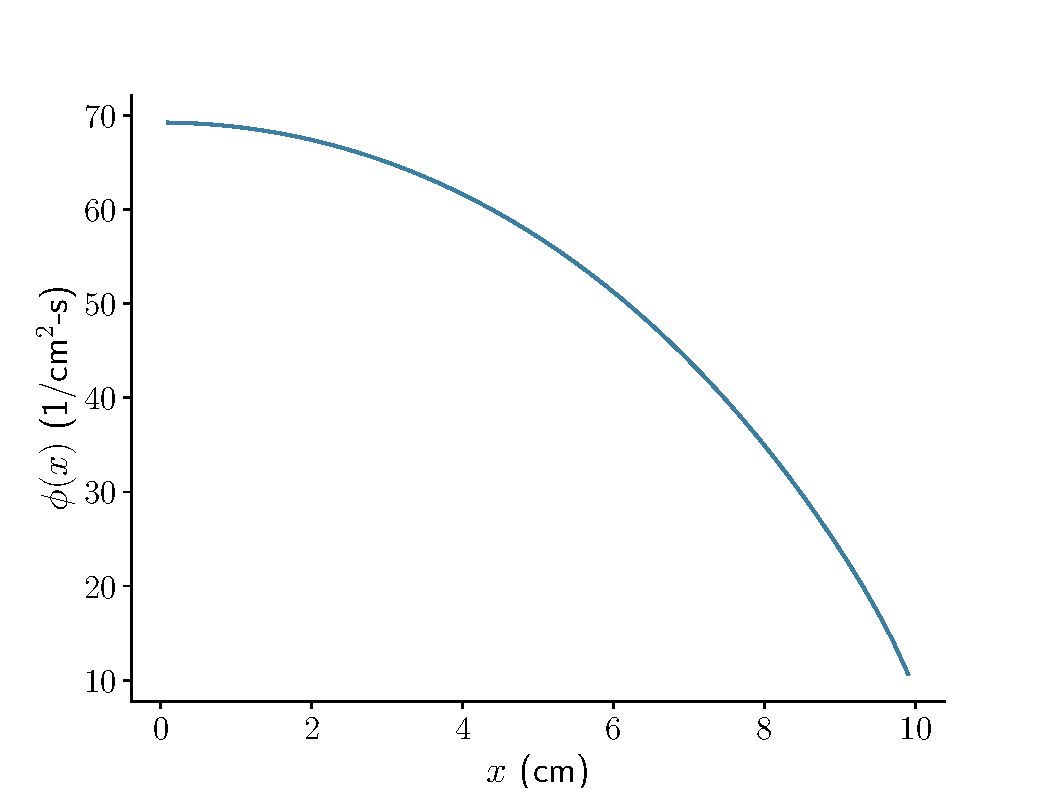
\includegraphics[width=.5\textwidth]{figs/phi_solution.pdf}
	\end{figure}

\end{frame}

\begin{frame}{Iterative Convergence Comparison}

	Relative iterative change (crude measure of iterative convergence)
	\begin{equation*}
		\frac{\| f^{\ell+1} - f^\ell \|_2}{\| f^{\ell+1} \|_2}
	\end{equation*}

	\vspace{-.2in}
	% \begin{figure}[htb]
	% \centering
	% \begin{subfigure}{.515\textwidth}
	% 	\centering
	% 	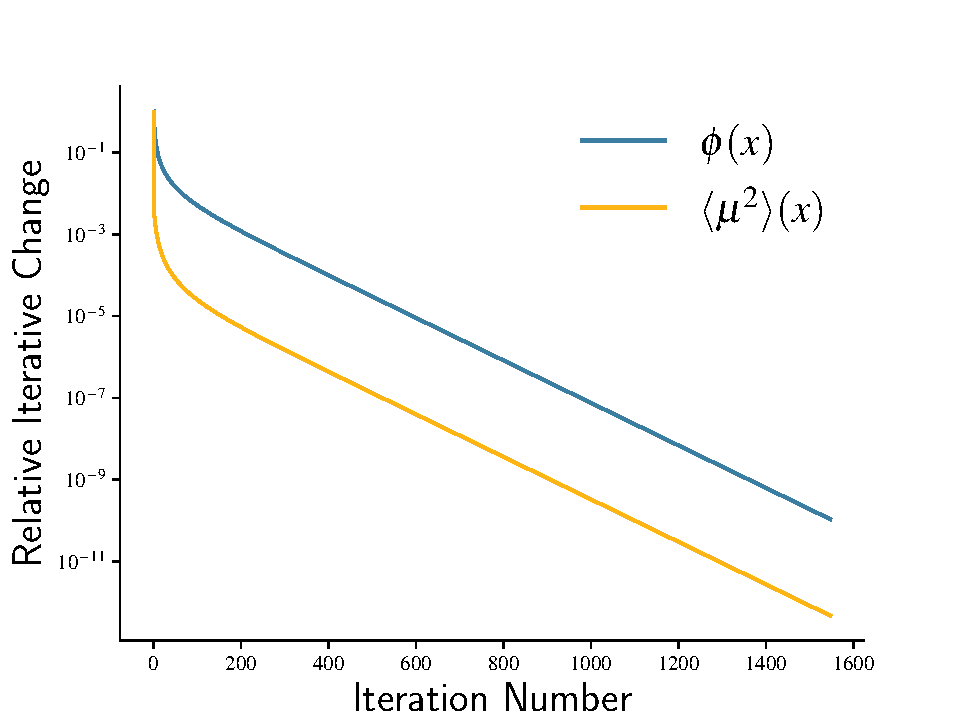
\includegraphics[width=\textwidth]{figs/si.pdf}
	% 	\caption{}
	% 	\label{fig:si}
	% \end{subfigure}
	% \hspace{-2em}
	% \begin{subfigure}{.515\textwidth}
	% 	\centering
	% 	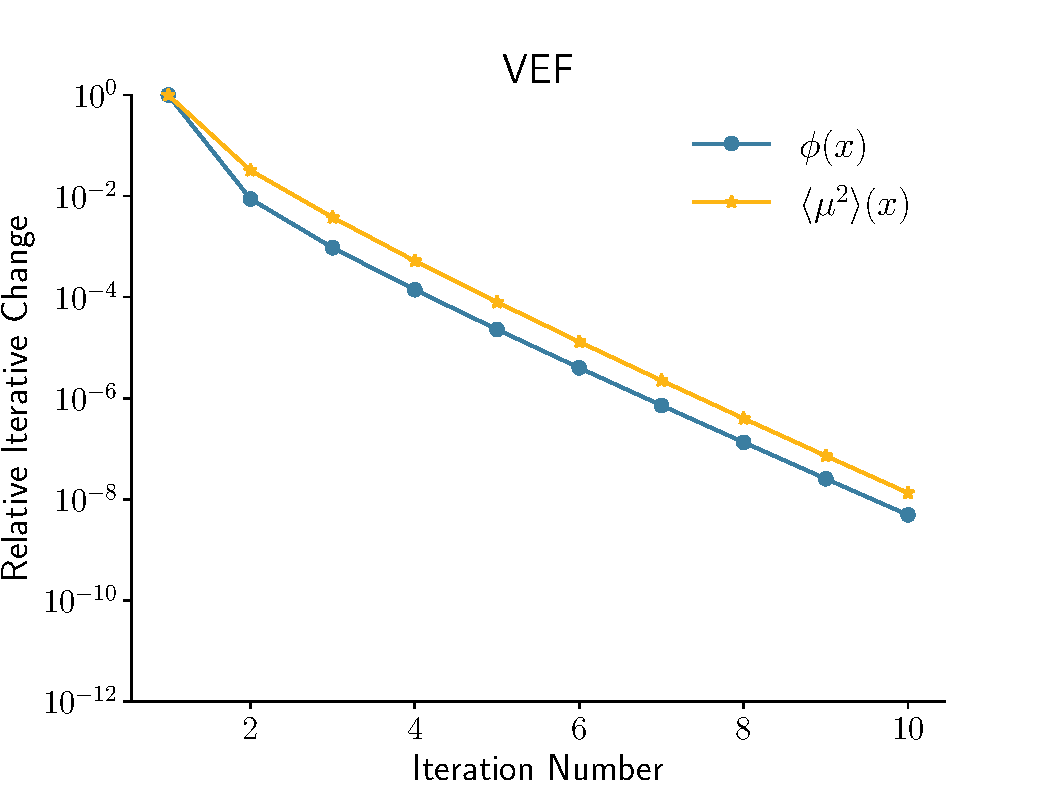
\includegraphics[width=\textwidth]{figs/vef.pdf}  
	% 	\caption{}
	% 	\label{fig:vef}
	% \end{subfigure}
	% \caption{Relative iterative change for $\phi(x)$ and $\edd(x)$ for (a) unaccelerated and (b) VEF accelerated SI. }
	% \end{figure}

	\begin{columns}

		\begin{column}{.55\textwidth}
		\begin{figure}
			\centering
			\onslide<1->{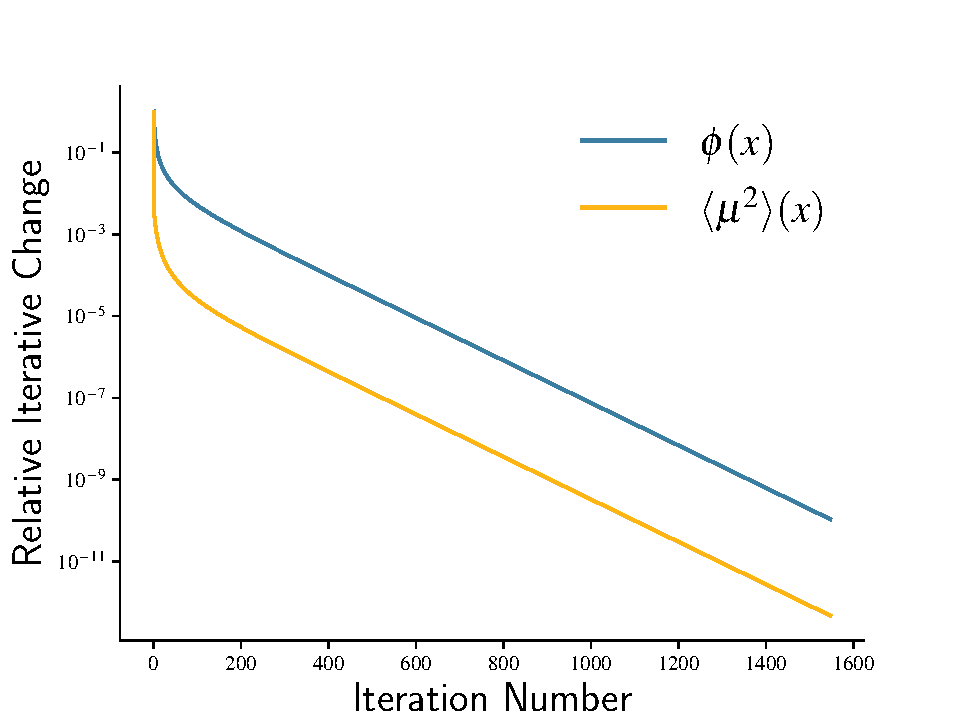
\includegraphics[width=\textwidth]{figs/si.pdf}}
		\end{figure}
		\end{column}
		\hspace{-2em}
		\begin{column}{.55\textwidth}
		\begin{figure}
			\centering
			\onslide<2->{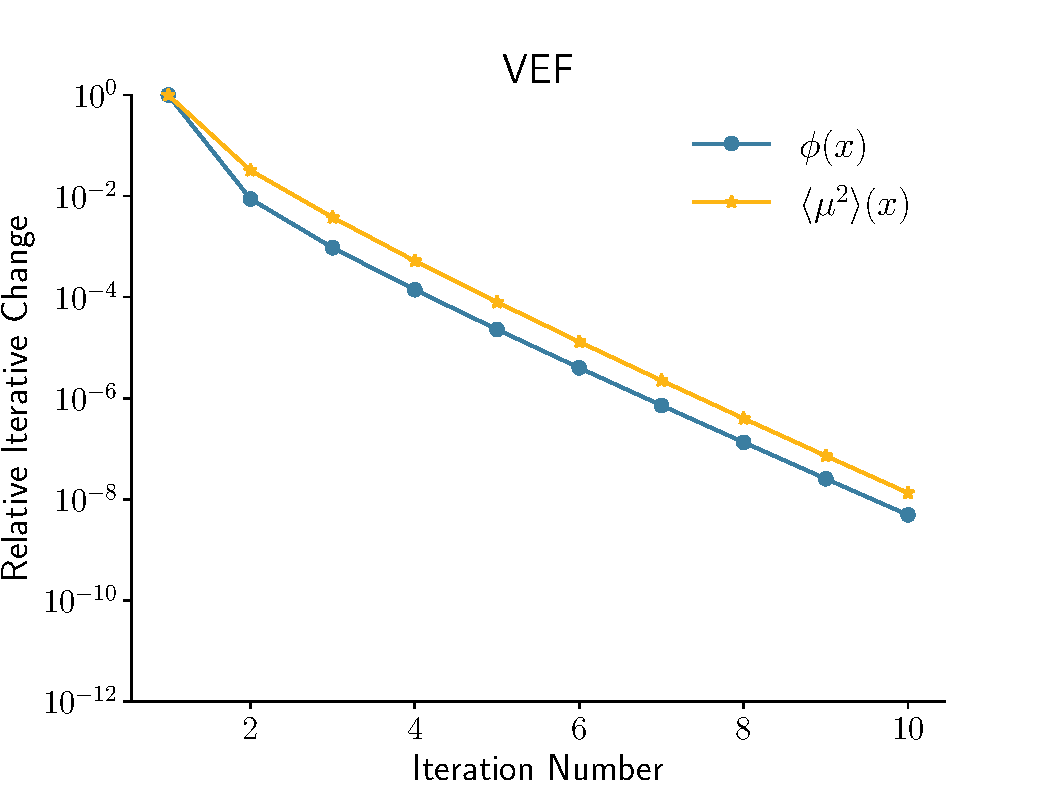
\includegraphics[width=\textwidth]{figs/vef.pdf}}
		\end{figure}
		\end{column}
	\end{columns}

	\vspace{.2in}
	\onslide<3->
	\begin{block}{}
	\centerline{Fast rate of convergence of $\edd(x)$ transfered to $\phi(x)$}
	\end{block}

\end{frame}

\begin{frame}{Comparison to SI and Consistently Differenced S$_2$SA}

	\begin{figure}[htb]
		\centering
		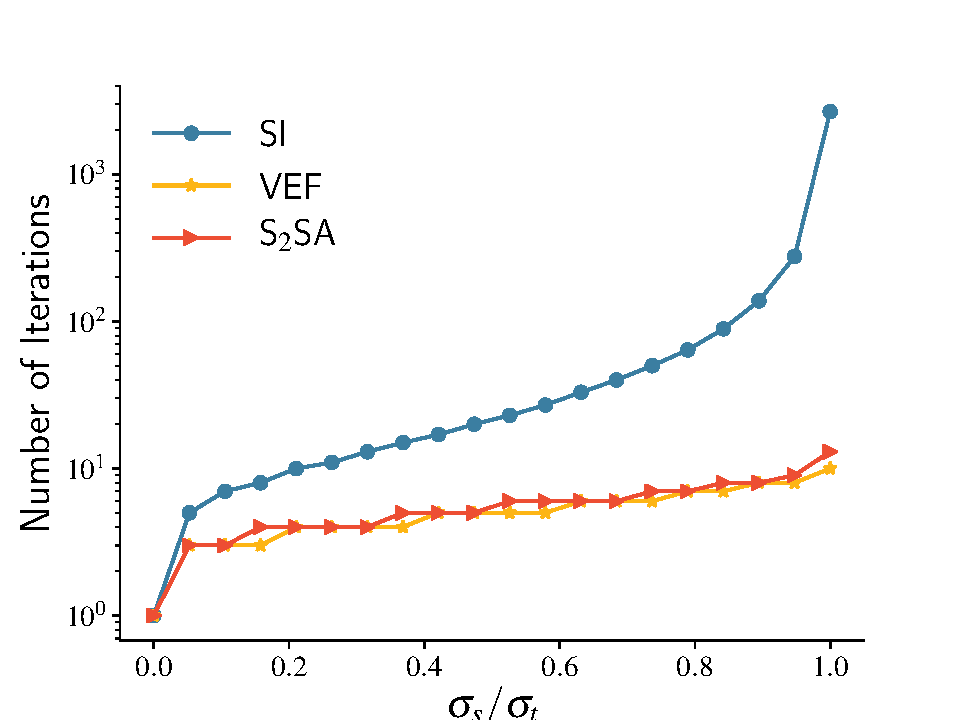
\includegraphics[width=.75\textwidth]{figs/si_vef_s2sa.pdf} 
		% \caption{A comparison of the number of iterations required to converge for Source Iteration, VEF acceleration, and S$_2$SA for varying ratios of $\sigma_s$ to $\sigma_t$. } 
		\label{fig:si_vef_s2sa}
	\end{figure}

	\begin{block}{}
		\centerline{VEF method performs similarly to consistently-differenced S$_2$SA}
	\end{block}

\end{frame}

\begin{frame}{Method of Manufactured Solutions}

	Set $Q(x, \mu_n)$ to force solution to 
	\begin{equation*}
		\phi(x) = \sin\left(\frac{\pi x}{x_b}\right)
	\end{equation*}

	Fit error to 
	\begin{equation*}
		E = C h^p 
	\end{equation*}

	\begin{table}[htb]
	\centering
	\begin{tabular}{|c|c|c|c|}
	\hline
	Update Method & $p$ & $C$ \\ 
	\hline
		Flat & \num{1.979} & \num{1.18} & \num{9.9999e-01} \\
Linear & \num{1.988} & \num{0.786} & \num{9.9887e-01} \\

	\hline
	\end{tabular}
	% \caption{The order of accuracy, error, and $R^2$ values for flat and linear slope reconstruction scattering source update methods. }
	\label{tab:mms}
	\end{table}

	\pause 
	\begin{block}{}
		\centering Same order of accuracy but linear reconstruction is more accurate 
	\end{block}

\end{frame}

\begin{frame}{VEF Drift Diffusion/\SN Solution Convergence}

	Compare the L$_2$ norm of the difference between \SN and drift diffusion solutions for:
	\begin{itemize} 

		\item Homogeneous system with $\frac{\sigma_s}{\sigma_t} = 0.99$ 

		\onslide<2->
		\item Reed's problem 

	\end{itemize}

	\begin{figure}
		\centering
		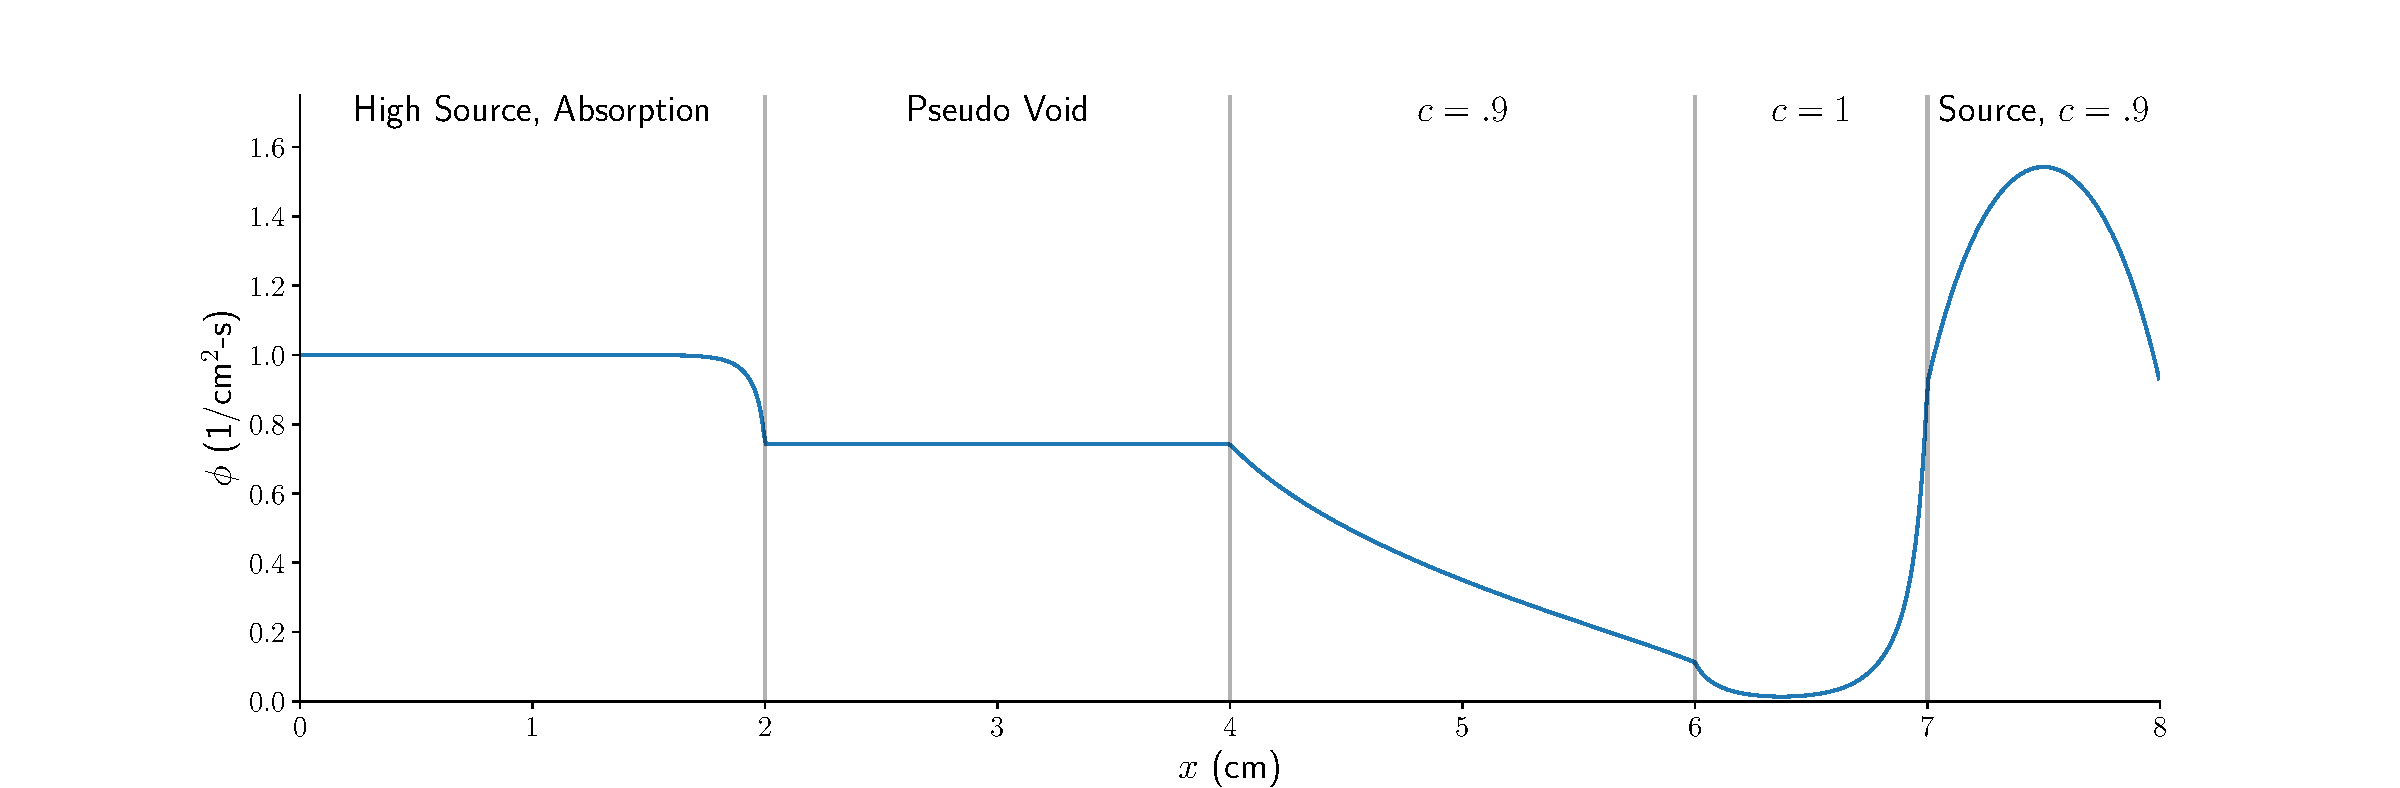
\includegraphics[width=\textwidth]{figs/reed_solution.pdf}
		% \caption{VEF solution for Reed's problem. }
	\end{figure}

\end{frame}

\begin{frame}{VEF Drift Diffusion/\SN Solution Convergence (cont.)}

	Compare 
		\begin{equation*}
			\frac{\|\phi_\text{Sn} - \phi_\text{VEF}\|}{\| \phi_\text{Sn}\|}
		\end{equation*}
	as cell spacing is decreased 

	\begin{figure}[htb]
		\centering
		\begin{subfigure}{.5\textwidth}
			\centering
			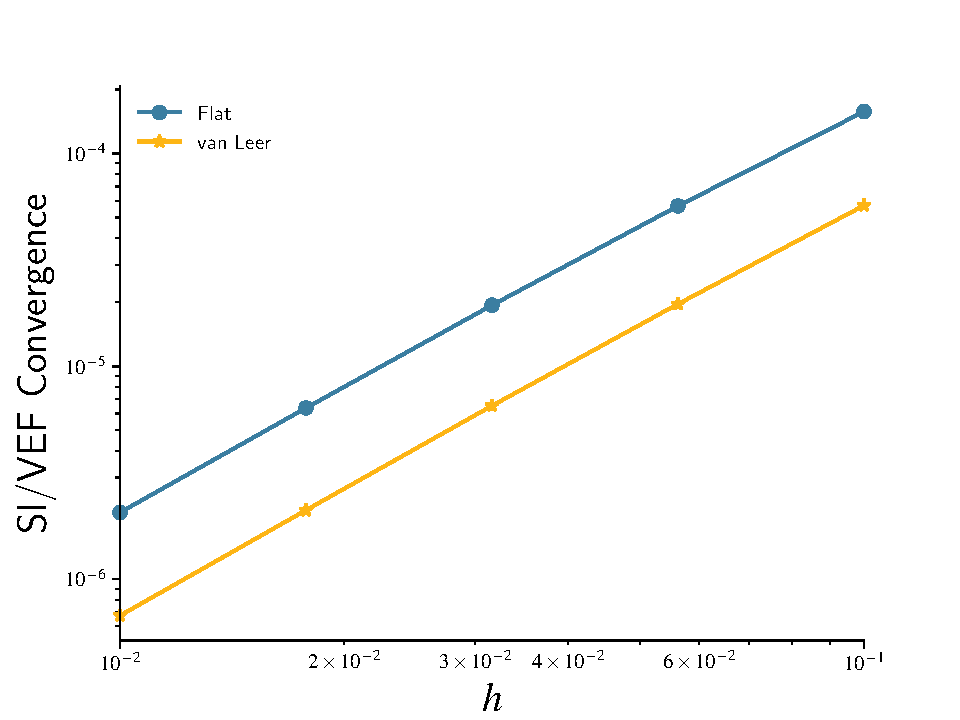
\includegraphics[width=\textwidth]{figs/solconv_homo.pdf}
			% \caption{}
			\label{fig:homo}
		\end{subfigure}
		\hspace{-2em}
		\begin{subfigure}{.5\textwidth}
			\centering
			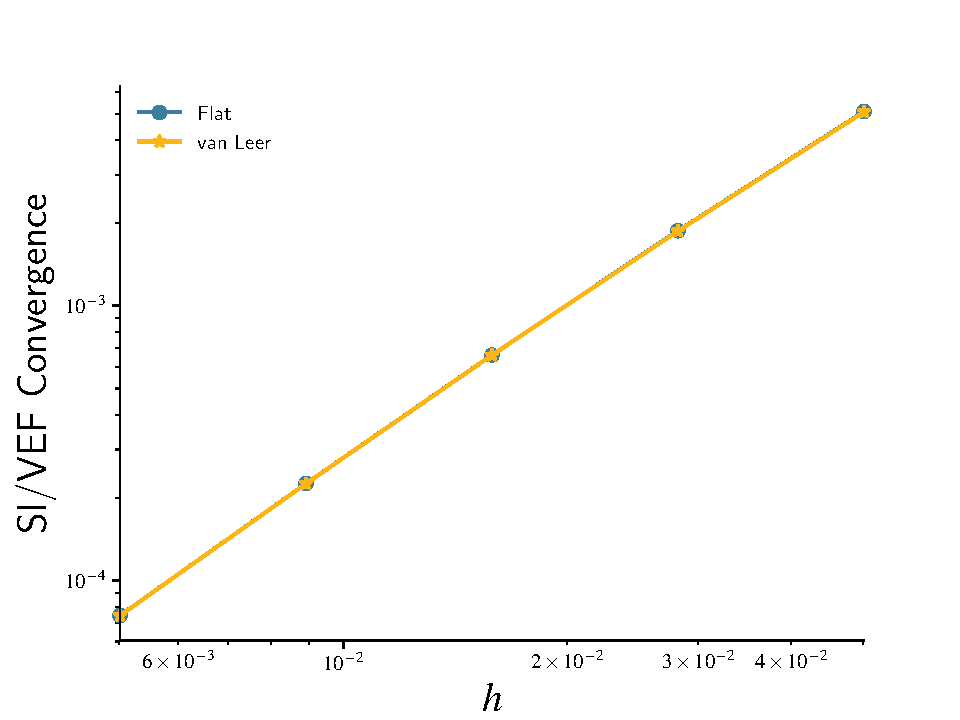
\includegraphics[width=\textwidth]{figs/solconv_reed.pdf}
			% \caption{}
			\label{fig:reed}
		\end{subfigure}
		% \caption{Comparison of difference between solutions for both scattering update methods for (a) homogeneous problem and (b) Reed's problem. }
	\end{figure}

	\pause
	\vspace{-.15in}
	% \begin{block}{}
	% 	\centering Linearly reconstructed solution is more accurate for homogeneous problem only 
	% \end{block}

	\SN and VEF solutions converge as mesh is refined (difference is $\propto$ LTE)

	\pause
	Linear reconstruction was 3 times as closer in homogeneous case but only 0.1\% more closer in Reed's problem 

\end{frame}

\begin{frame}{Thick Diffusion Limit Test}

	Scale cross sections and source according to:
	$$ \sigma_t(x) \rightarrow \sigma_t(x)/\epsilon, \ $$
	$$ \sigma_a(x) \rightarrow \epsilon \sigma_a(x), \ $$
	$$ Q(x) \rightarrow \epsilon Q(x) $$

	Diffusion length is invariant 
	\begin{equation*}
		L^2 = \frac{D}{\sigma_a} = \frac{1}{3\sigma_t\sigma_a} \rightarrow
			\frac{1}{3 \frac{\sigma_t}{\epsilon} \sigma_a \epsilon}
	\end{equation*}

	As $\epsilon \rightarrow 0$, the system becomes diffusive 

\end{frame}

\begin{frame}{Thick Diffusion Limit Test (cont.)}

	\begin{columns}
	\begin{column}{.5\textwidth}
		\begin{figure}[htb]
			\centering
			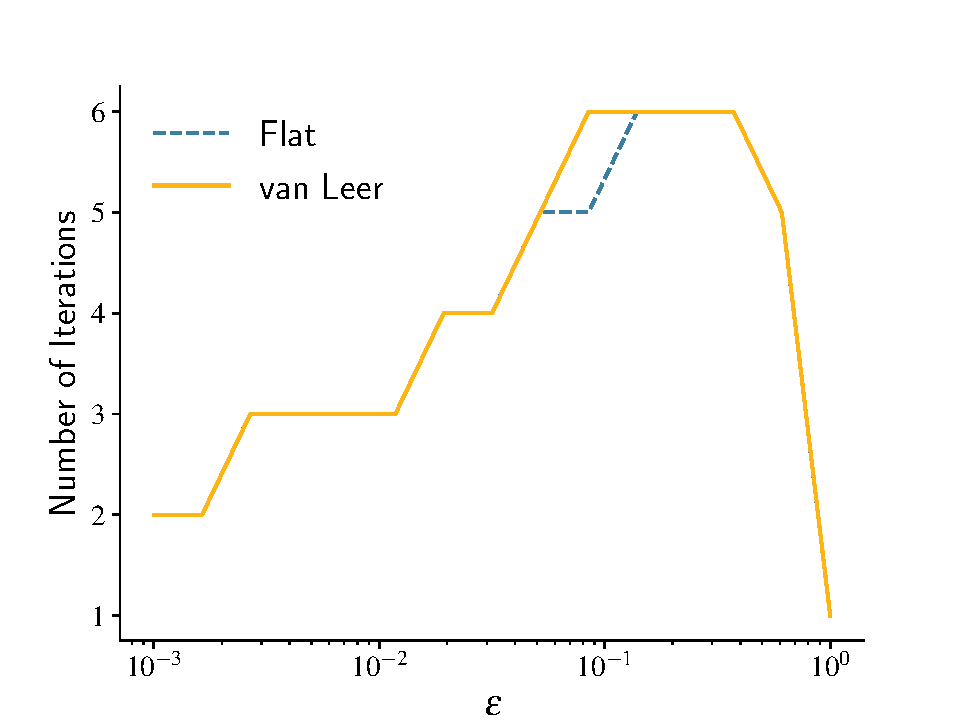
\includegraphics[width=1.05\textwidth]{figs/dl_it.pdf}
			% \caption{The number of iterations required for convergence in the diffusion limit ($\epsilon \rightarrow 0$). }
			\label{fig:dl_it}
		\end{figure}
	\end{column}
	\begin{column}{.5\textwidth}
		\begin{figure}
			\centering
			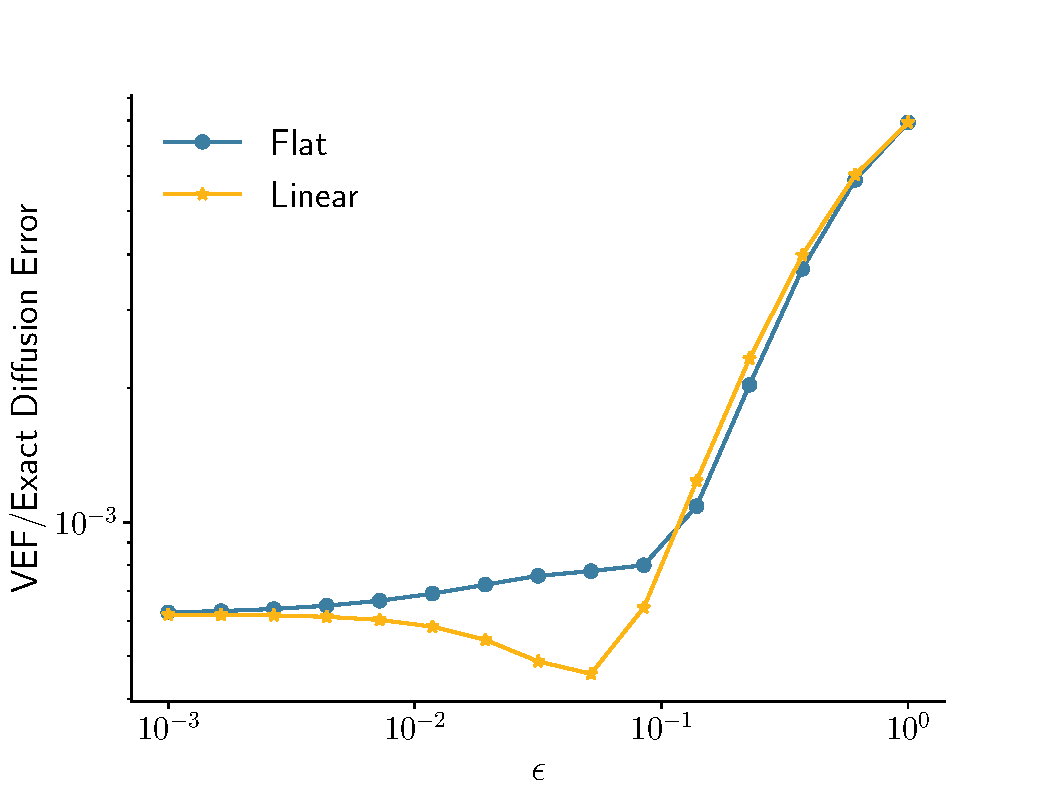
\includegraphics[width=1.05\textwidth]{figs/dl_err.pdf}
			% \caption{The error between the VEF methods and the exact diffusion solution as $\epsilon \rightarrow 0$. }
			\label{fig:dl_err}
		\end{figure}
	\end{column}
	\end{columns}

	\pause
	VEF solution $\rightarrow$ exact diffusion as $\epsilon \rightarrow 0$

	\pause 
	Inconsistent discretization still preserves acceleration in thick diffusion limit 


\end{frame}

\section{Conclusions and Future Work }

\begin{frame}{Conclusions}

	Successfully paired Lumped Linear Discontinuous Galerkin \SN with constant-linear Mixed Finite Element drift diffusion 

	Acceleration is as effective as consistently differenced S$_2$SA 

	Thick diffusion limit is preserved 

	Overlap between discretizations:
	\begin{itemize}
		\item Carried linear dependence from LLDG into MFEM 

		\item Used slope reconstruction with limiting to regenerate a linear \SN source from MFEM 

	\end{itemize}

	Conservative drift diffusion equation can be coupled to other physics components

	Drift diffusion discretization can match other physics components while retaining benefits of DG \SN 

	Built in error estimator 

\end{frame}

\begin{frame}{Future Work}

	Extend to high order finite elements in 2/3D 

	Radiative transfer 

	Investigate the impact of the linear reconstruction method on the "teleportation effect"

\end{frame}


% begin uncounted slides ---------------------------
\appendix

\begin{frame}[allowframebreaks]{References}

	\nocite{*}
	\setbeamerfont{bibliography item}{size=\scriptsize}
	\setbeamerfont{bibliography entry author}{size=\scriptsize}
	\setbeamerfont{bibliography entry title}{size=\scriptsize}
	\setbeamerfont{bibliography entry location}{size=\scriptsize}
	\setbeamerfont{bibliography entry note}{size=\scriptsize}
	\setbeamertemplate{bibliography item}{\insertbiblabel}
	\bibliographystyle{siam}
	\bibliography{references}

\end{frame}

\begin{frame}[standout]
  Questions?
\end{frame}

\end{document}
